\chapter{Produire notre nourriture}\label{ch:g6:producing-our-food}

Rien de ce qui est sur ta table du petit déjeuner n'a été trouvé
dans la nature. Le blé du pain a été sélectionné et cultivé~; le
\omterm{def:g2:animals-grow-up:born}{lait} vient de troupeaux élevés pour cela~; le yaourt a été
\emph{fabriqué} à partir de ce \omterm{def:g2:animals-grow-up:born}{lait} par des milliards d'ouvriers
vivants trop petits pour être vus. Les humains se nourrissent en
gérant des \omterm{def:g6:exploring-our-environment:components}{êtres vivants} --- en les cultivant, en les élevant, et en
mettant certains des plus petits au travail. Ce chapitre visite
l'atelier alimentaire.

\section{Cultiver et élever}

\begin{definition}[Cultures et élevage]\label{def:g6:producing-our-food:farming}
La production alimentaire humaine gère des \omterm{def:g6:exploring-our-environment:components}{êtres vivants} à deux
étages du cycle de la matière~:
\begin{itemize}
  \item la \emph{culture}\index{culture}~: gérer des \omterm{def:g5:food-webs:roles}{producteurs}
        --- blé, pommes de terre, légumes, \omterm{prop:g3:flowers-fruits-seeds:transform}{fruits} --- pour leur
        \omterm{def:g6:plants-are-producers:matter}{matière organique}
        (\cref{prop:g6:plants-are-producers:produce})~;
  \item l'\emph{élevage}\index{élevage}~: gérer des \omterm{def:g5:food-webs:roles}{consommateurs}
        --- bovins, moutons, cochons, poules --- pour leur
        \omterm{def:g6:matter-from-food:production}{production de matière}
        (\cref{def:g6:matter-from-food:production})~: \omterm{def:g2:animals-grow-up:born}{lait}, viande,
        \omterm{def:g2:animals-grow-up:born}{œufs}, laine.
\end{itemize}
Les agriculteurs gèrent les \omterm{def:g6:exploring-our-environment:conditions}{conditions} que ce livre ne cesse de
rencontrer~: les minéraux du \omterm{def:g6:decomposers-and-soil:soil}{sol} pour les cultures
(\cref{rem:g4:what-plants-need:soil}), l'alimentation pour les
\omterm{def:g1:animals-around-us:animal}{animaux} --- tout le registre de
\cref{pb:g6:matter-from-food:1}, tenu à dessein.
\end{definition}

\begin{example}[Ce qu'est un champ de blé]\label{ex:g6:producing-our-food:wheat}
Un champ de blé est un \omterm{def:g6:exploring-our-environment:components}{environnement} géré
(\cref{prop:g5:people-and-nature:managed}) réglé pour un seul
\omterm{def:g5:food-webs:roles}{producteur}~: \omterm{def:g6:decomposers-and-soil:soil}{sol} réapprovisionné et ameubli pour ses \omterm{def:g1:plants-around-us:parts}{racines}, semis
calé sur la chaleur de \cref{prop:g2:from-seed-to-plant:needs},
mauvaises herbes --- colons rivaux de
\cref{ch:g6:how-plants-spread} --- tenues dehors. La récolte est la
réserve de \omterm{prop:g3:flowers-fruits-seeds:transform}{graines} de la \omterm{def:g1:plants-around-us:plant}{plante}~: du grain, les casse-croûte
emballés d'un million de pieds de blé qui ne seront jamais semés,
détournés vers les boulangeries.
\end{example}

\begin{remark}[Tout aliment est un stade d'un cycle de vie]\label{rem:g6:producing-our-food:stage}
Lis n'importe quel aliment en biologiste et c'est l'organe ou le
stade d'un organisme~: le grain et les haricots sont des réserves de
\omterm{prop:g3:flowers-fruits-seeds:transform}{graines}~; les pommes de terre, des \omterm{ex:g4:plants-without-seeds:bulbtuber}{tubercules}~; les pommes, des
\omterm{prop:g3:flowers-fruits-seeds:transform}{fruits} bâtis pour être mangés
(\cref{exo:g6:how-plants-spread:12})~; le \omterm{def:g2:animals-grow-up:born}{lait} est un soin maternel
de mammifère (\cref{def:g2:animals-grow-up:born})~; un \omterm{def:g2:animals-grow-up:born}{œuf} est une
nurserie garnie. Produire de la nourriture est l'art de gérer des
\omterm{def:g2:born-grow-die:cycle}{cycles de vie} pour que leurs provisions arrivent sur nos tables.
\end{remark}

\section{La main-d'œuvre invisible~: des aliments faits par des microbes}

\begin{definition}[Fermentation]\label{def:g6:producing-our-food:fermentation}
Certains aliments sont fabriqués en mettant au travail sur une
matière première des \omterm{def:g6:exploring-our-environment:components}{êtres vivants} trop petits pour être vus --- les
\emph{microbes}\index{microbe (alimentation)}. Leur alimentation la
transforme~: cette transformation s'appelle la
\emph{fermentation}\index{fermentation}, et les humains la mènent
depuis des milliers d'années, bien avant que quiconque ait su que
les ouvriers existaient.
\end{definition}

\begin{example}[Le pain lève]\label{ex:g6:producing-our-food:bread}
La pâte crue du pain, c'est de la farine et de l'eau --- plus de la
\emph{levure}\index{levure}, un \omterm{def:g6:decomposers-and-soil:decomposers}{champignon} à une seule \omterm{def:g5:first-look-at-cells:cell}{cellule}
(\cref{rem:g5:first-look-at-cells:onecelled} avait rencontré de
telles vies). La \omterm{ex:g6:producing-our-food:bread}{levure} se nourrit des sucres de la farine et
libère un gaz~; les bulles de ce gaz, piégées dans la pâte
élastique, la gonflent --- le boulanger appelle cela la pousse. La
chaleur du four met ensuite fin au service des ouvriers et fige leur
travail~: les trous de la mie sont la signature de la \omterm{ex:g6:producing-our-food:bread}{levure}.
\end{example}

\begin{omfigure}
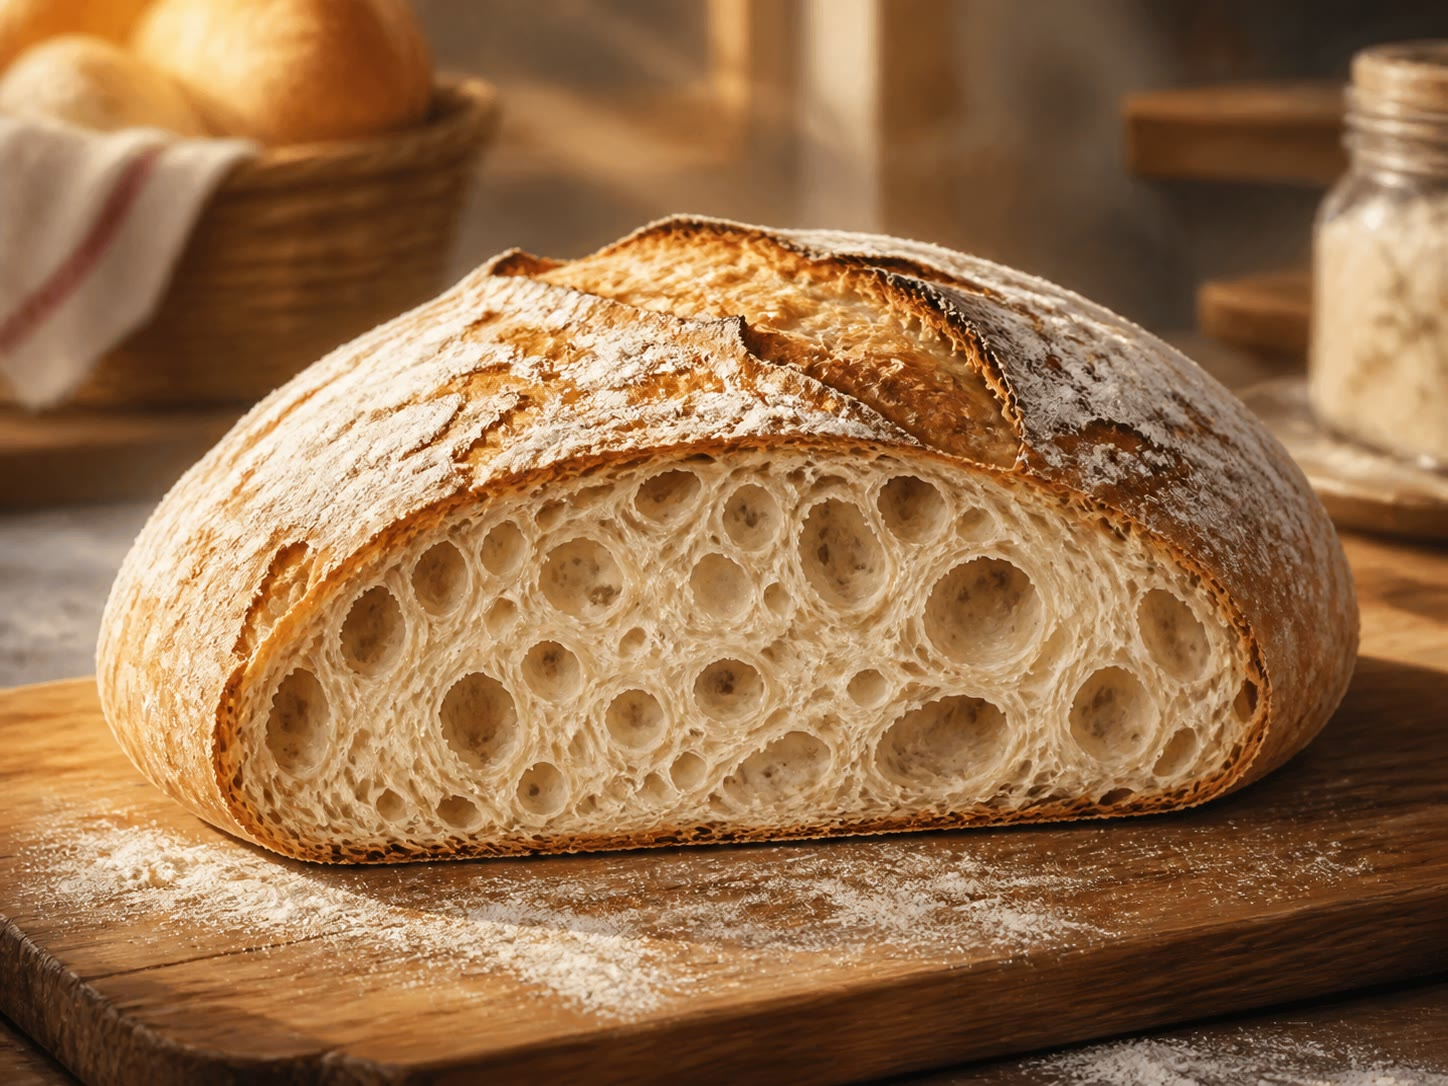
\includegraphics[width=0.58\linewidth]{images/book1/ai/g6-food-bread.jpg}

{\small La signature de la main-d'œuvre, cuite sur place~: chaque
trou de la mie est une bulle soufflée par la \omterm{ex:g6:producing-our-food:bread}{levure}.}
\end{omfigure}

\begin{example}[Le lait devient yaourt et fromage]\label{ex:g6:producing-our-food:yogurt}
Du \omterm{def:g2:animals-grow-up:born}{lait} tiède ensemencé des bons \omterm{def:g6:producing-our-food:fermentation}{microbes} s'épaissit en une nuit en
yaourt~: les ouvriers se nourrissent du sucre du \omterm{def:g2:animals-grow-up:born}{lait} et libèrent un
acide, et l'acide fait prendre le \omterm{def:g2:animals-grow-up:born}{lait} --- le goût frais et acidulé
\emph{est} cet acide. Le fromage commence de la même façon, puis va
plus loin~: caillé pressé, salé et affiné pendant des mois, les
\omterm{def:g6:producing-our-food:fermentation}{microbes} travaillant tout au long de l'affinage --- les trous, la
croûte et la puissance d'odeur d'un fromage sont le journal de leur
long service.
\end{example}

\begin{remark}[Microbes utiles et microbes nuisibles]\label{rem:g6:producing-our-food:goodbad}
Les \omterm{def:g6:producing-our-food:fermentation}{microbes} de \cref{def:g1:healthy-habits:germs} enseignaient la
prudence~; ce chapitre en ajoute l'autre moitié~: des \omterm{def:g6:producing-our-food:fermentation}{microbes}
\emph{choisis}, travaillant dans des \omterm{def:g6:exploring-our-environment:conditions}{conditions}
\emph{contrôlées}, comptent parmi nos plus anciens employés --- dans
le pain, le yaourt, le fromage et le tonneau de vinaigre. Le
savoir-faire est toujours le même~: accueillir les ouvriers choisis,
et maintenir des \omterm{def:g6:exploring-our-environment:conditions}{conditions} qui leur conviennent et pas aux
gâcheurs. Saler, refroidir, sécher et cuire sont autant de façons de
refuser leurs \omterm{def:g6:exploring-our-environment:conditions}{conditions} aux \omterm{def:g6:producing-our-food:fermentation}{microbes} indésirables
(\cref{prop:g6:decomposers-and-soil:speed} vaut pour un jambon
exactement comme pour un tas de \omterm{def:g1:plants-around-us:parts}{feuilles}).
\end{remark}

\section{Du champ à la table, honnêtement}

\begin{proposition}[Ce que coûte une assiette]\label{prop:g6:producing-our-food:costs}
Toute assiette est le produit de terres et d'\omterm{def:g6:exploring-our-environment:components}{êtres vivants} gérés, et
elle en porte l'arithmétique~:
\begin{itemize}
  \item les aliments végétaux arrivent à un étage de la \omterm{def:g6:exploring-our-environment:conditions}{lumière}~;
        les aliments \omterm{def:g1:animals-around-us:animal}{animaux} passent d'abord par un \omterm{def:g5:food-webs:roles}{consommateur} et
        paient le péage de
        \cref{prop:g6:matter-from-food:losses}
        (\cref{exo:g6:matter-from-food:12})~;
  \item une production durable doit respecter les trois règles de
        \cref{prop:g5:people-and-nature:lasting} --- nourrir le
        \omterm{def:g6:decomposers-and-soil:soil}{sol}, garder les auxiliaires, ne pas prélever plus vite que
        le renouvellement~;
  \item et le gaspillage défait tout~: un aliment jeté a dépensé sa
        terre, son eau et son travail pour personne.
\end{itemize}
\end{proposition}
\admitted

\begin{method}[Lire l'histoire d'un aliment]\label{met:g6:producing-our-food:read}
Pour n'importe quel aliment de la cuisine~:
\begin{enumerate}
  \item nomme l'organisme, et l'organe ou le stade dont il s'agit
        (\cref{rem:g6:producing-our-food:stage})~;
  \item place-le sur le cycle~: matière d'un \omterm{def:g5:food-webs:roles}{producteur}, production
        d'un \omterm{def:g5:food-webs:roles}{consommateur}, ou fabrication de \omterm{def:g6:producing-our-food:fermentation}{microbes}~?
  \item si ce sont des \omterm{def:g6:producing-our-food:fermentation}{microbes}, nomme la matière première et ce
        que les ouvriers ont changé~;
  \item retrace-le jusqu'à sa \omterm{def:g1:plants-around-us:parts}{feuille}
        (\cref{met:g6:plants-are-producers:trace}) --- la piste se
        termine toujours dans la \omterm{def:g6:exploring-our-environment:conditions}{lumière}.
\end{enumerate}
\end{method}

\begin{example}[La méthode au petit déjeuner]\label{ex:g6:producing-our-food:breakfast}
Le yaourt, par la méthode~: (1) du \omterm{def:g2:animals-grow-up:born}{lait} --- une production de soin
maternel de vache --- transformé~; (2) production d'un \omterm{def:g5:food-webs:roles}{consommateur},
achevée par des \omterm{def:g6:producing-our-food:fermentation}{microbes}~; (3) matière première~: le \omterm{def:g2:animals-grow-up:born}{lait}, que les
ouvriers ont acidifié et fait prendre~; (4) le \omterm{def:g2:animals-grow-up:born}{lait} vient de la
vache, la vache de l'herbe, l'herbe de la \omterm{def:g6:exploring-our-environment:conditions}{lumière}. Trois organismes
et une main-d'œuvre de milliards, dans un petit pot.
\end{example}

\section{Exercices}

\begin{exercise}[$\star$]\label{exo:g6:producing-our-food:1}
Définis la \omterm{def:g6:producing-our-food:farming}{culture} et l'\omterm{def:g6:producing-our-food:farming}{élevage}, en nommant l'étage du cycle de la
matière que chacun gère.
\end{exercise}

\begin{exercise}[$\star$]\label{exo:g6:producing-our-food:2}
Pour chaque aliment, nomme l'organisme et l'organe ou le stade~: le
grain, la pomme de terre, la pomme, le \omterm{def:g2:animals-grow-up:born}{lait}, l'\omterm{def:g2:animals-grow-up:born}{œuf}.
\end{exercise}

\begin{exercise}[$\star$]\label{exo:g6:producing-our-food:3}
Qu'est-ce que la \omterm{def:g6:producing-our-food:fermentation}{fermentation}~? Nomme deux aliments fermentés et
leurs matières premières.
\end{exercise}

\begin{exercise}[$\star$]\label{exo:g6:producing-our-food:4}
Explique pourquoi le pain lève~: l'ouvrier, sa nourriture, ce qu'il
libère, et ce que fait le four.
\end{exercise}

\begin{exercise}[$\star$]\label{exo:g6:producing-our-food:5}
Qu'est-ce qui fait prendre le \omterm{def:g2:animals-grow-up:born}{lait} en yaourt, et d'où vient le goût
acidulé~?
\end{exercise}

\begin{exercise}[$\star$]\label{exo:g6:producing-our-food:6}
Donne trois façons de refuser leurs \omterm{def:g6:exploring-our-environment:conditions}{conditions} aux \omterm{def:g6:producing-our-food:fermentation}{microbes}
indésirables, d'après \cref{rem:g6:producing-our-food:goodbad}.
\end{exercise}

\begin{exercise}[$\star\star$]\label{exo:g6:producing-our-food:7}
Un champ de blé gère à dessein chacun des besoins de
\cref{prop:g4:what-plants-need:needs}. Associe chaque besoin à
l'action de l'agriculteur décrite dans
\cref{ex:g6:producing-our-food:wheat}.
\end{exercise}

\begin{exercise}[$\star\star$]\label{exo:g6:producing-our-food:8}
Applique \cref{met:g6:producing-our-food:read} au fromage, étape
par étape.
\end{exercise}

\begin{exercise}[$\star\star$]\label{exo:g6:producing-our-food:9}
Pourquoi la réfrigération conserve-t-elle les aliments --- et
pourquoi le même froid ralentit-il un tas de compost~? Un seul
principe, deux cuisines~: nomme-le.
\end{exercise}

\begin{exercise}[$\star\star$]\label{exo:g6:producing-our-food:10}
Concilie \cref{def:g1:healthy-habits:germs} avec ce chapitre~:
comment les \omterm{def:g6:producing-our-food:fermentation}{microbes} peuvent-ils être à la fois l'ennemi du lavage
des mains et la main-d'œuvre du yaourt~?
\end{exercise}

\begin{exercise}[$\star\star$]\label{exo:g6:producing-our-food:11}
À l'aide de \cref{prop:g6:producing-our-food:costs}, explique
pourquoi un sandwich au jambon jeté gaspille davantage que le même
poids de pain jeté.
\end{exercise}

\begin{exercise}[$\star\star\star$]\label{exo:g6:producing-our-food:12}
Pendant des milliers d'années, boulangers et brasseurs ont mené la
\omterm{def:g6:producing-our-food:fermentation}{fermentation} sans savoir que les \omterm{def:g6:producing-our-food:fermentation}{microbes} existaient. Qu'ont-ils
géré en réalité, dans les termes de
\cref{prop:g6:exploring-our-environment:decide} --- et pourquoi
leurs recettes marchaient-elles quand même~?
\end{exercise}

\section{Problème~: la boulangerie de la classe}

\begin{problem}[{Problème du week-end --- une fournée de pain,
suivie de la graine à la tranche}]\label{pb:g6:producing-our-food:1}
Pour la fête de l'école, la classe cuit du pain de A à Z --- et
tient son carnet de \omterm{def:g1:living-or-not:living}{biologie} ouvert depuis la visite du champ de blé
en juillet jusqu'aux miches de novembre.

\medskip\noindent\textbf{Partie I --- Le champ (juillet).}
\begin{enumerate}
  \item L'agriculteur montre le blé mûr~: «~la récolte, ce sont les
        casse-croûte emballés de la \omterm{def:g1:plants-around-us:plant}{plante}~». Déplie la formule
        avec \cref{def:g2:from-seed-to-plant:seed} --- qu'est-ce
        que chaque grain, et pour qui a-t-il été emballé~?
  \item Dans les \omterm{def:g1:plants-around-us:parts}{feuilles} de qui, et avec quelles entrées, la
        \omterm{def:g6:plants-are-producers:matter}{matière organique} du grain a-t-elle été fabriquée~?
  \item L'agriculteur ne sème qu'une partie de la récolte l'automne
        suivant et vend le reste. Nomme les deux destins d'un grain
        de blé, en termes de \omterm{def:g2:born-grow-die:cycle}{cycle de vie}.
  \item Le \omterm{def:g6:decomposers-and-soil:soil}{sol} du champ reçoit du fumier après la récolte. De
        quelle règle de retour s'agit-il, et lequel des cinq
        besoins de la \omterm{def:g1:plants-around-us:plant}{plante} sert-elle~?
\end{enumerate}

\medskip\noindent\textbf{Partie II --- La boulangerie (novembre).}
\begin{enumerate}[resume]
  \item La classe mélange farine, eau, sel et \omterm{ex:g6:producing-our-food:bread}{levure}, et pose la
        pâte dans un coin chaud. Pourquoi chaud~? Réponds pour la
        \omterm{ex:g6:producing-our-food:bread}{levure} comme pour n'importe quel ouvrier vivant
        (\cref{prop:g6:decomposers-and-soil:speed} donne le
        modèle).
  \item Une heure plus tard, la pâte a doublé. Explique la pousse~:
        de quoi la \omterm{ex:g6:producing-our-food:bread}{levure} s'est-elle nourrie, qu'a-t-elle libéré,
        et qu'est-ce qui l'a piégé~?
  \item La pâte d'une équipe, oubliée près d'une fenêtre froide et
        pleine de courants d'air, lève à peine. Fais le diagnostic
        --- et dis quelle comparaison d'expérience honnête les deux
        équipes ont menée sans le vouloir.
  \item Au four, les miches cessent de lever et figent. Qu'a fait
        la chaleur à la main-d'œuvre, et que reste-t-il de sa
        signature dans la mie~?
\end{enumerate}

\medskip\noindent\textbf{Partie III --- La comptabilité.}
\begin{enumerate}[resume]
  \item Retrace la tranche finie jusqu'à la \omterm{def:g6:exploring-our-environment:conditions}{lumière}, maillon par
        maillon.
  \item La fête vend aussi du beurre et des sandwichs au jambon.
        Classe la tranche, le beurre et le jambon selon les étages
        que leur matière a traversés, et dis lequel a payé le plus
        gros péage de
        \cref{prop:g6:matter-from-food:losses}.
  \item La pâte invendue est compostée, pas jetée. Suis sa \omterm{def:g6:plants-are-producers:matter}{matière
        organique} d'un tour de plus autour du cycle --- qui la
        prend, et vers quoi~?
  \item Referme le carnet avec une phrase contenant~: \omterm{def:g5:food-webs:roles}{producteur},
        \omterm{def:g5:food-webs:roles}{consommateur} (s'il y en a un), main-d'œuvre de \omterm{def:g6:producing-our-food:fermentation}{microbes} et
        \omterm{def:g6:exploring-our-environment:conditions}{lumière}.
\end{enumerate}
\end{problem}
